
\section{Aufbau}
\label{sec:Aufbau}

\begin{wrapfigure}[23]{r}{7cm}
\vspace{-0.5cm}
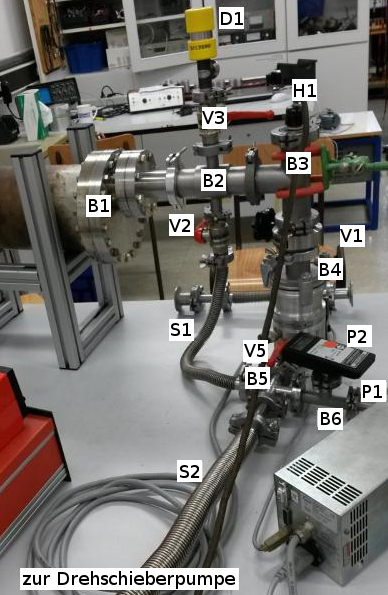
\includegraphics[scale=0.5]{content/images/Aufbau2.jpg}
\caption{Aufbau zum Experiment Vakuumphysik \cite{V70}.}
\label{fig:Aufbau}
\end{wrapfigure}

Der Versuch wird wie in Abbildung \ref{fig:Aufbau} aufgebaut. Am Rezipient B1 wird über ein Kreuzstück ein Nadelventil (D1) für die Leckratenmessung der Drehschieberpumpe und alle Messungen der Turbomolekularpumpe angebracht, das über ein Kugelventil komplett geschlossen werden kann. Über ein T-Stück wird ein Kaltkathoden-Vakuummeter, das in der Abbildung nicht zu sehen ist, angeschlossen und der Rezipient über ein weiteres T-Stück mit eingebautem Heizkathoden-Vakuummeter (H1) und ein Klappenventil (V1) mit der Turbopumpe verbunden. Mit einem weiteren Kugelventil (V2) wird der Tank außerdem über die Schläuche S1 und S2 direkt mit der Drehschieberpumpe verbunden, die außerdem zur Erzeugung des Vorvakuums mit der Turbopumpe und einem analogen und einem digitalen Pirani-Vakuummeter (P1 und P2) verbunden. Letzteres war bei dieser Durchführung des Versuchs defekt.


